\chapter{Ellingham Diagrams and Metallurgy}\label{ch:b2:ellingham}

A blast furnace turns red rock into liquid iron with coke and hot air, at a
rate of thousands of tonnes a day. No furnace of that kind will ever make
aluminium, magnesium or titanium, although carbon is just as cheap for them.
Most metals are found in the ground as oxides, and winning a metal means
taking its oxygen away: which reducing agents can do it, and at what
temperature, is a question of standard Gibbs energies. In 1944 Harold
Ellingham drew them all on one chart, against temperature, for one mole of
dioxygen each. The chart answers at a glance which metal reduces which oxide,
why carbon wins at high temperature, and why some metals must be made by
electrolysis.

\begin{recall}
\Cref{ch:b2:reaction-free-energy}: $\Delta_r G^\circ = \Delta_r H^\circ -
T\Delta_r S^\circ$ and the \omterm{def:b2:reaction-free-energy:ellingham-approximation}{Ellingham approximation} (straight lines in $T$,
changes of state excepted). \Cref{ch:b2:equilibrium-shifts}: $K^\circ$ from
$\Delta_r G^\circ$, \omterm{def:b2:equilibrium-shifts:variance}{variance}, the end of an equilibrium when a phase
disappears. The Year 1 volume: oxidation numbers, redox couples, basic and
acidic oxides. The school volume: ores.
\end{recall}

\begin{omfigure}
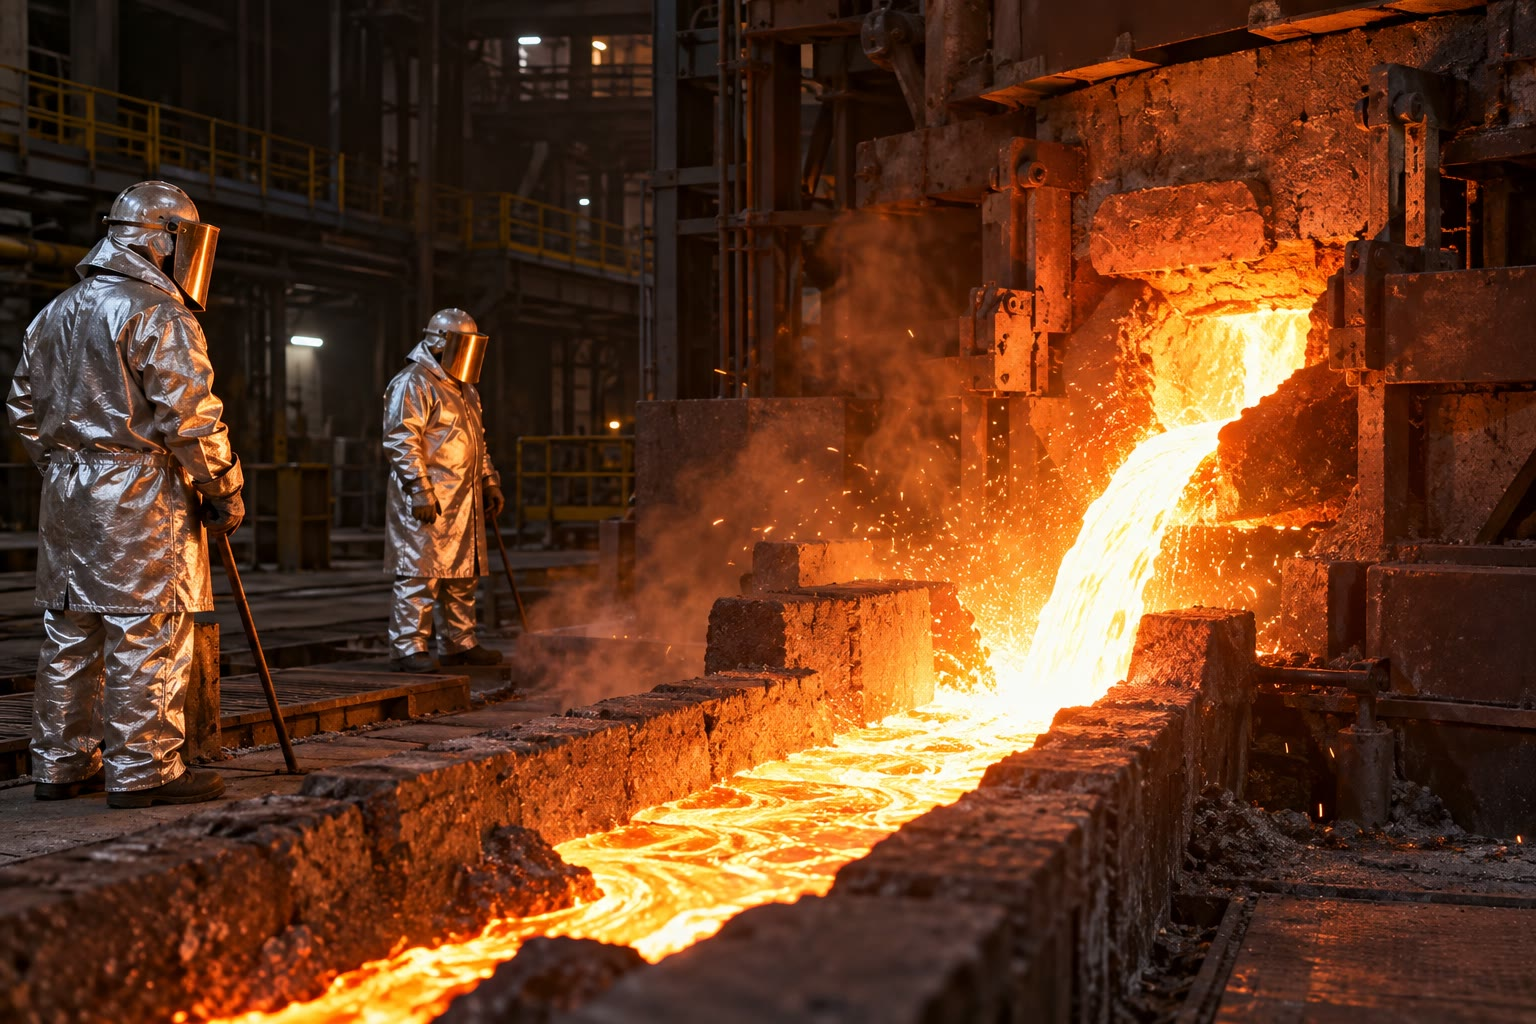
\includegraphics[width=0.62\linewidth]{images/book3/ai/b2-06-blast-furnace.jpg}

{\small Tapping a blast furnace: liquid iron runs along a refractory channel,
watched by workers in heat-reflecting suits. The temperature and the gas
inside the furnace are those that let carbon monoxide take the oxygen away
from iron oxide.}
\end{omfigure}

\section{The Ellingham diagram}

To compare the affinity of different metals for oxygen, the reactions are
written so that they all consume the same amount of the common reagent.

\begin{definition}[Ellingham diagram]\label{def:b2:ellingham:diagram}
The \emph{Ellingham diagram}\index{Ellingham diagram} of a family of oxides
is the graph, against temperature, of the standard Gibbs energies of their
formation reactions written for one mole of dioxygen,
\[
  \tfrac{2x}{y}\,\mathrm M + \ce{O2} \longrightarrow \tfrac{2}{y}\,\mathrm{M}_x\mathrm O_y ,
  \qquad \Delta_r G^\circ(T) \ \text{per mole of } \ce{O2} .
\]
\end{definition}

For example \ce{2Zn + O2 -> 2ZnO}, \ce{4/3Al + O2 -> 2/3Al2O3}, \ce{2C + O2 ->
2CO}. The ordinate is in \unit{kJ} per mole of \ce{O2}, always negative for the
metals of the chart.

\begin{proposition}[Straight lines]\label{prop:b2:ellingham:line}
In the \omterm{def:b2:reaction-free-energy:ellingham-approximation}{Ellingham approximation}, each line is straight, of slope $-\Delta_r
S^\circ$. For a metal and its oxide, both condensed, $\Delta_r S^\circ$ is
close to minus the entropy of the mole of dioxygen consumed, about
$-\qty{200}{J/(K.mol)}$: the lines rise with temperature, all with nearly the
same slope.
\end{proposition}

\begin{proof}
$\Delta_r G^\circ = \Delta_r H^\circ - T\Delta_r S^\circ$ with constant $\Delta_r
H^\circ$, $\Delta_r S^\circ$. The molar entropies of solids are tens of
\unit{J/(K.mol)} and largely cancel between metal and oxide, while one mole of
gas is consumed, of entropy $S^\circ(\ce{O2}) = \qty{205}{J/(K.mol)}$. For zinc,
$2(43.65) - 2(41.63) - 205.15 = \qty{-201.1}{J/(K.mol)}$.
% ledger: s0:ZnO_cr, s0:Zn_cr, s0:O2_g
\end{proof}

\begin{proposition}[Breaks in the lines]\label{prop:b2:ellingham:break}
At the temperature where the metal melts or boils, the line changes slope:
its slope increases by $\nu\,\Delta_{\text{trs}}S$, where $\nu$ is the amount of
metal in the reaction and $\Delta_{\text{trs}}S = \Delta_{\text{trs}}H/T_{\text{trs}}$.
A change of state of the oxide decreases the slope instead.
\end{proposition}

\begin{proof}
Above the transition the metal reacts from its new phase, whose entropy is
higher by $\Delta_{\text{trs}}S$: $\Delta_r S^\circ$ decreases by $\nu\,\Delta_{\text{trs}}S$
and the slope $-\Delta_r S^\circ$ increases by as much. $\Delta_r G^\circ$
itself is continuous, because at $T_{\text{trs}}$ both phases have the same
\omterm{def:b2:chemical-potential:chemical-potential}{chemical potential}. For the oxide, the opposite sign.
\end{proof}

Melting changes the slope a little; boiling, which turns a condensed reactant
into a gas, changes it a lot. Zinc boils at \qty{1180}{K}: above that
temperature the formation of zinc oxide consumes three moles of gas per two of
oxide, and its line climbs steeply. The same happens to magnesium above its
boiling point.

\begin{omfigure}
\begin{tikzpicture}[lab/.style={anchor=west, font=\scriptsize, inner sep=1pt}]
\begin{axis}[omellingham,
  width=0.84\linewidth, height=11cm, xmin=300, xmax=2100, ymin=-1250, ymax=0,
  clip mode=individual,
  xlabel={$T$ (K)}, ylabel={$\Delta_r G^\circ$ (\unit{kJ} per mol \ce{O2})},
  xtick={300,500,700,900,1100,1300,1500,1700,1900,2100},
  x tick label style={rotate=45, anchor=north east, font=\scriptsize}]
\addplot[black!60, thick] table[x=T, y=G] {figdata/out/bachelor-2-ellingham-a-HgO.dat};
\addplot[omProp, thick] table[x=T, y=G] {figdata/out/bachelor-2-ellingham-a-Cu2O.dat};
\addplot[omDef, thick] table[x=T, y=G] {figdata/out/bachelor-2-ellingham-a-FeO.dat};
\addplot[omExo, very thick] table[x=T, y=G] {figdata/out/bachelor-2-ellingham-a-ZnO.dat};
\addplot[black!60, thick] table[x=T, y=G] {figdata/out/bachelor-2-ellingham-a-Cr2O3.dat};
\addplot[omProp, thick] table[x=T, y=G] {figdata/out/bachelor-2-ellingham-a-TiO2.dat};
\addplot[omDef, thick] table[x=T, y=G] {figdata/out/bachelor-2-ellingham-a-Al2O3.dat};
\addplot[black!60, thick] table[x=T, y=G] {figdata/out/bachelor-2-ellingham-a-MgO.dat};
\addplot[omProp, thick] table[x=T, y=G] {figdata/out/bachelor-2-ellingham-a-CaO.dat};
\addplot[omThm, very thick] table[x=T, y=G] {figdata/out/bachelor-2-ellingham-a-C-CO.dat};
\addplot[omThm, thick, dashed] table[x=T, y=G] {figdata/out/bachelor-2-ellingham-a-C-CO2.dat};
\addplot[omThm, thick, dotted] table[x=T, y=G] {figdata/out/bachelor-2-ellingham-a-CO-CO2.dat};
\addplot[omDef, thick, dashed] table[x=T, y=G] {figdata/out/bachelor-2-ellingham-a-H2-H2O.dat};
% labels: inside for the two short lines, at the right end for the others
\node[font=\scriptsize, black!70, anchor=south] at (axis cs:400,-60) {\ce{HgO}};
\node[font=\scriptsize, omProp, anchor=south] at (axis cs:1100,-150) {\ce{Cu2O}};
\draw[omExo, thin] (axis cs:2100,-69) -- (axis cs:2150,-60) node[lab, text=omExo] {\ce{ZnO}};
\draw[omThm, thin] (axis cs:2100,-204) -- (axis cs:2150,-185) node[lab, text=omThm] {\ce{CO}/\ce{CO2}};
\draw[omDef, thin] (axis cs:2100,-259) -- (axis cs:2150,-235) node[lab, text=omDef] {\ce{H2}/\ce{H2O}};
\draw[omDef, thin] (axis cs:2100,-286) -- (axis cs:2150,-285) node[lab, text=omDef] {\ce{FeO}};
\draw[black!70, thin] (axis cs:2100,-393) -- (axis cs:2150,-365) node[lab, text=black!70] {\ce{Cr2O3}};
\draw[omThm, thin] (axis cs:2100,-396) -- (axis cs:2150,-415) node[lab, text=omThm] {\ce{C}/\ce{CO2}};
\draw[omProp, thin] (axis cs:2100,-567) -- (axis cs:2150,-540) node[lab, text=omProp] {\ce{TiO2}};
\draw[omThm, thin] (axis cs:2100,-589) -- (axis cs:2150,-590) node[lab, text=omThm] {\ce{C}/\ce{CO}};
\draw[black!70, thin] (axis cs:2100,-600) -- (axis cs:2150,-640) node[lab, text=black!70] {\ce{MgO}};
\draw[omDef, thin] (axis cs:2100,-668) -- (axis cs:2150,-690) node[lab, text=omDef] {\ce{Al2O3}};
\draw[omProp, thin] (axis cs:2100,-765) -- (axis cs:2150,-765) node[lab, text=omProp] {\ce{CaO}};
\end{axis}
\end{tikzpicture}

{\small The \omterm{def:b2:ellingham:diagram}{Ellingham diagram}: standard \omterm{def:b2:reaction-free-energy:gibbs-energy}{Gibbs energy} of formation of oxides
per mole of \ce{O2}, against temperature, from tabulated Gibbs energies. The
lower a line, the more stable the oxide and the more reducing the metal.
Each metal line is labelled by its oxide; \ce{C}/\ce{CO} is \ce{2C + O2 -> 2CO},
\ce{C}/\ce{CO2} is \ce{C + O2 -> CO2}, \ce{CO}/\ce{CO2} is \ce{2CO + O2 -> 2CO2}
and \ce{H2}/\ce{H2O} is \ce{2H2 + O2 -> 2H2O}, water as a gas.}
% ledger: janafG:Cu2O.300, janafG:FeO.300, janafG:Cr2O3.300, janafG:TiO2.500, janafG:Al2O3.300, janafG:MgO.300, janafG:CaO.300, janafG:CO.300, janafG:CO2.300, janafG:H2O.300, dfh:ZnO_cr, dfh:HgO_cr, s0:HgO_cr, s0:Hg_l, s0:Hg_g, dfh:Hg_g (all temperatures in figdata/bachelor-2/ellingham.py)
\end{omfigure}

\section{Reading the diagram}

\begin{definition}[Equilibrium oxygen pressure]\label{def:b2:ellingham:oxygen-pressure}
The \emph{equilibrium oxygen pressure}\index{equilibrium oxygen pressure} of a
metal–oxide pair at temperature $T$ is the pressure of dioxygen at which metal
and oxide coexist at equilibrium: $RT\ln(p_{\ce{O2}}/p^\circ) = \Delta_r
G^\circ(T)$ for the reaction written per mole of \ce{O2}.
\end{definition}

\begin{theorem}[Domains of the metal and of the oxide]\label{thm:b2:ellingham:domains}
In an atmosphere of oxygen pressure $p_{\ce{O2}}$ at temperature $T$, the
metal is oxidised if $RT\ln(p_{\ce{O2}}/p^\circ) > \Delta_r G^\circ(T)$, and the
oxide is reduced to the metal if $RT\ln(p_{\ce{O2}}/p^\circ) < \Delta_r
G^\circ(T)$. On the diagram, the oxide is stable above its line, the metal
below.
\end{theorem}

\begin{proof}
With condensed metal and oxide of activity 1, $Q = p^\circ/p_{\ce{O2}}$ and
$\Delta_r G = \Delta_r G^\circ + RT\ln Q = \Delta_r G^\circ - RT\ln(p_{\ce{O2}}/
p^\circ)$. The oxidation runs forward when $\Delta_r G < 0$.
\end{proof}

Under air ($p_{\ce{O2}} = \qty{0.21}{bar}$, $RT\ln 0.21$ is \qty{-4}{kJ/mol}
at room temperature and \qty{-13}{kJ/mol} at \qty{1000}{K}, almost zero on this
scale) every metal of the diagram whose line
is below the axis is oxidised: at room temperature all of them, even copper.
Only the oxides near the top (silver, mercury) decompose on moderate
heating.

\begin{example}[The oxide of mercury]\label{ex:b2:ellingham:hgo}
For \ce{2Hg + O2 -> 2HgO}, the CODATA key values give $\Delta_r H^\circ =
\qty{-181.6}{kJ/mol}$ with liquid mercury; above the boiling point of mercury
the metal is a gas and $\Delta_r H^\circ = \qty{-304.3}{kJ/mol}$, $\Delta_r
S^\circ = \qty{-414.6}{J/(K.mol)}$. The line crosses zero at
$T = 304.3/0.4146 \approx \qty{734}{K}$: heated above that temperature in air,
or under \qty{1}{bar} of oxygen, red mercury oxide gives off its oxygen ---
the way oxygen was first isolated in 1774.
% ledger: dfh:HgO_cr, s0:HgO_cr, s0:Hg_l, s0:Hg_g, dfh:Hg_g, s0:O2_g (computed in figdata/bachelor-2/ellingham.py)
\end{example}

\begin{proposition}[Which metal reduces which oxide]\label{prop:b2:ellingham:reduction}
At a given temperature, a metal M reduces the oxide of a metal N, under
standard conditions, when the line of M lies below that of N. The \omterm{def:b2:reaction-free-energy:reaction-gibbs}{standard
reaction Gibbs energy} of the reduction, per mole of \ce{O2} transferred, is the
difference of the two ordinates.
\end{proposition}

\begin{proof}
The reduction is the formation of M's oxide minus that of N's oxide, both per
mole of \ce{O2}: $\Delta_r G^\circ = \Delta_r G^\circ_{\mathrm M} - \Delta_r
G^\circ_{\mathrm N}$, negative when M's line is lower.
\end{proof}

\begin{method}[Reading an Ellingham diagram]\label{met:b2:ellingham:read-ellingham}
\begin{enumerate}
  \item Find the two lines at the temperature of interest. The lower one is
        the more stable oxide; its metal reduces the other oxide.
  \item The vertical gap is $\Delta_r G^\circ$ per mole of \ce{O2}: a gap of
        \qty{100}{kJ} or more means a practically complete reduction.
  \item Where two lines cross, the reduction changes direction: read the
        crossing temperature.
  \item Watch the breaks: a metal that boils inside the interval leaves as a
        vapour, which can be distilled off --- or which reoxidises on cooling.
\end{enumerate}
\end{method}

\begin{definition}[Aluminothermic reduction]\label{def:b2:ellingham:aluminothermy}
An \emph{aluminothermic reduction}\index{aluminothermic reduction} is the
reduction of a metal oxide by aluminium powder, possible for every oxide whose
line lies above that of alumina, and so \omterm{def:b2:reaction-enthalpy:exothermic}{exothermic} that the mixture melts:
\ce{Fe2O3 + 2Al -> Al2O3 + 2Fe} (thermite) welds rails; \ce{Cr2O3 + 2Al ->
Al2O3 + 2Cr} makes chromium free of carbon.
\end{definition}

\begin{omfigure}
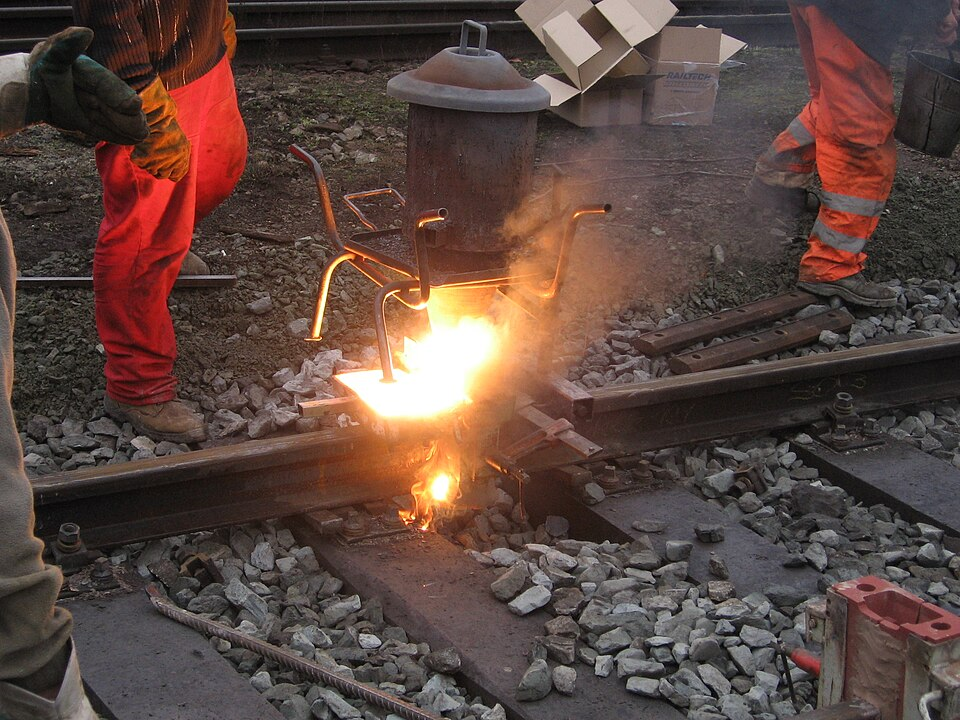
\includegraphics[width=0.5\linewidth]{images/book3/thermite.jpg}

{\small Thermite welding of a rail: the reaction of iron oxide with aluminium
in the crucible above the joint gives liquid iron, which runs down into the
mould between the two rail ends. (Photograph: PetrS., CC BY-SA 3.0, Wikimedia
Commons.)}
\end{omfigure}

\section{Carbon and carbon monoxide}

Three lines involve carbon:
\begin{itemize}
  \item \ce{C + O2 -> CO2}: one mole of gas gives one, $\Delta_r S^\circ
        \approx 0$, an almost horizontal line near \qty{-395}{kJ};
  \item \ce{2C + O2 -> 2CO}: one mole of gas gives two, $\Delta_r S^\circ
        \approx \qty{+180}{J/(K.mol)}$, a line that \emph{falls} with temperature;
  \item \ce{2CO + O2 -> 2CO2}: three moles of gas give two, a rising line.
\end{itemize}

\begin{proposition}[Carbon reduces almost everything when hot]\label{prop:b2:ellingham:carbon}
The line of \ce{2C + O2 -> 2CO} decreases with temperature and crosses the
lines of most metal oxides: above the crossing temperature, carbon reduces the
oxide, giving carbon monoxide. The crossing for iron(II) oxide is near
\qty{1040}{K}, for zinc oxide near \qty{1220}{K}; for titania and magnesia it
lies near or above \qty{2000}{K}, for alumina higher still, where the metals
combine with carbon into carbides or reoxidise as the gas cools.
\end{proposition}

\begin{proof}
The slope $-\Delta_r S^\circ$ of the carbon line is negative ($\Delta\nu_{\text{gas}}
= +1$), that of the oxide lines positive: they meet once. The temperatures
are read on the computed lines.
% ledger: janafG:CO.900, janafG:CO.1100, janafG:FeO.900, janafG:FeO.1100 (crossings computed in figdata/bachelor-2/ellingham.py)
\end{proof}

\begin{definition}[Boudouard equilibrium]\label{def:b2:ellingham:boudouard}
The \emph{Boudouard equilibrium}\index{Boudouard equilibrium} is \ce{C(s) + CO2(g) <=> 2CO(g)},
\omterm{def:b2:reaction-enthalpy:exothermic}{endothermic}, between carbon and the two oxides of carbon.
\end{definition}

\begin{proposition}[Composition of the gas over carbon]\label{prop:b2:ellingham:boudouard}
The system carbon + \ce{CO} + \ce{CO2} has \omterm{def:b2:equilibrium-shifts:variance}{variance} 2: at a given $T$ and total
pressure $p$, the mole fraction $x$ of carbon monoxide is fixed by $x^2/(1 - x)
= K^\circ(T)\,p^\circ/p$. At \qty{1}{bar} the gas is almost pure \ce{CO2}
below \qty{700}{K} and almost pure \ce{CO} above \qty{1200}{K}; the crossing of
the three carbon lines, near \qty{975}{K}, is where $K^\circ = 1$.
\end{proposition}

\begin{proof}
Three species, one reaction, two phases: $v = 3 - 1 + 2 - 2 = 2$. With $p_{\ce{CO}}
= xp$ and $p_{\ce{CO2}} = (1 - x)p$, $Q = x^2p/[(1 - x)p^\circ]$. At $K^\circ = 1$,
the standard Gibbs energies of \ce{2C + O2 -> 2CO} and \ce{C + O2 -> CO2} are
equal: the two lines, and so the third, meet.
\end{proof}

\begin{omfigure}
\begin{tikzpicture}
\begin{axis}[
  width=0.62\linewidth, height=5.4cm, xmin=500, xmax=1500, ymin=0, ymax=1.05,
  axis x line=bottom, axis y line=left, xlabel={$T$ (K)},
  xtick={500,700,900,1100,1300,1500}, ytick={0,0.5,1},
  ylabel={mole fraction of \ce{CO}}, tick label style={font=\small},
  label style={font=\small}, clip=false]
\addplot[omThm, very thick] table[x=T, y=xCO] {figdata/out/bachelor-2-ellingham-b.dat};
\node[font=\scriptsize, anchor=west] at (axis cs:1150,0.55) {\ce{CO} stable};
\node[font=\scriptsize, anchor=west] at (axis cs:510,0.6) {\ce{CO2} (and carbon) stable};
\end{axis}
\end{tikzpicture}

{\small The \omterm{def:b2:ellingham:boudouard}{Boudouard equilibrium} at \qty{1}{bar}: mole fraction of carbon
monoxide in a gas in equilibrium with carbon.}
% ledger: janafG:CO.700, janafG:CO2.700, janafG:CO.1100, janafG:CO2.1100 (computed in figdata/bachelor-2/ellingham.py)
\end{omfigure}

\section{The blast furnace}

Iron ore (hematite \ce{Fe2O3}, magnetite \ce{Fe3O4}), coke and limestone are
charged at the top of a tall shaft; hot air is blown in
near the bottom. Going down, the solids meet a hot rising gas; the gas leaves
at the top, cooled.
\begin{itemize}
  \item At the tuyeres, coke burns in the hot air: \ce{C + O2 -> CO2}, and
        above, with excess carbon, \ce{CO2 + C -> 2CO} (Boudouard): the gas
        that rises is mostly carbon monoxide and nitrogen.
  \item In the upper part, carbon monoxide reduces the iron oxides step by
        step, \ce{3Fe2O3 + CO -> 2Fe3O4 + CO2}, \ce{Fe3O4 + CO -> 3FeO + CO2},
        \ce{FeO + CO -> Fe + CO2}. The first two steps are easy; for the last,
        the \ce{CO}/\ce{CO2} line runs a little \textit{above} the line of
        \ce{FeO}: its \omterm{def:b2:reaction-free-energy:reaction-gibbs}{standard reaction Gibbs energy} is slightly positive
        ($K^\circ \approx 0.3$ at \qty{900}{K}), and the reduction needs a gas
        holding at least three times more \ce{CO} than \ce{CO2} --- which the
        \omterm{def:b2:ellingham:boudouard}{Boudouard equilibrium} supplies in the hot zone below.
  \item Lower and hotter, carbon itself reduces what remains, \ce{FeO + C ->
        Fe + CO}; the iron dissolves carbon, melts, and collects at the bottom
        with a molten slag formed by lime and the silica of the ore.
\end{itemize}

\begin{omfigure}
\begin{tikzpicture}[font=\small, >={Stealth}]
  \fill[gray!12] (-1.4,0) -- (-2.0,3.0) -- (-1.3,7.0) -- (1.3,7.0) -- (2.0,3.0) -- (1.4,0) -- cycle;
  \draw[thick] (-1.4,0) -- (-2.0,3.0) -- (-1.3,7.0) (1.4,0) -- (2.0,3.0) -- (1.3,7.0);
  \draw[thick] (-1.4,0) -- (1.4,0);
  \fill[orange!70!red] (-1.4,0) rectangle (1.4,0.35);
  \fill[yellow!50!orange] (-1.45,0.35) rectangle (1.45,0.6);
  \node[font=\scriptsize] at (0,0.17) {liquid iron};
  \node[font=\scriptsize] at (0,0.48) {slag};
  % tuyeres
  \draw[->, thick, omDef] (-3.2,1.2) -- (-1.75,1.2) node[pos=0, left] {hot air};
  \draw[->, thick, omDef] (3.2,1.2) -- (1.75,1.2);
  % charge and gas
  \draw[->, thick] (-0.6,7.9) -- (-0.6,7.1) node[pos=0, above left, xshift=6pt] {ore, coke, limestone};
  \draw[->, thick, omThm] (0.7,7.1) -- (0.7,7.9) node[pos=1, above right, xshift=-6pt] {top gas (\ce{CO}, \ce{CO2}, \ce{N2})};
  \draw[->, omThm, thick] (0.6,1.6) -- (0.6,6.4);
  \draw[->, thick] (-0.6,6.4) -- (-0.6,1.6);
  \node[omThm, font=\scriptsize, rotate=90] at (0.9,4.0) {gas rises};
  \node[font=\scriptsize, rotate=90] at (-0.9,4.0) {solids descend};
  % zones
  \node[anchor=west, align=left, font=\scriptsize] at (2.3,6.0) {\ce{3Fe2O3 + CO -> 2Fe3O4 + CO2}\\ \ce{Fe3O4 + CO -> 3FeO + CO2}};
  \node[anchor=west, align=left, font=\scriptsize] at (2.3,4.2) {\ce{FeO + CO -> Fe + CO2}};
  \node[anchor=west, align=left, font=\scriptsize] at (2.3,2.7) {\ce{CO2 + C -> 2CO}\\ \ce{FeO + C -> Fe + CO}};
  \node[anchor=west, align=left, font=\scriptsize] at (2.3,1.6) {\ce{C + O2 -> CO2}};
  \draw[densely dotted] (1.95,6.0) -- (2.3,6.0) (1.9,4.2) -- (2.3,4.2) (2.0,2.8) -- (2.3,2.8);
  \node[anchor=east, align=right, font=\scriptsize, black!60] at (-2.2,6.0) {cooler};
  \node[anchor=east, align=right, font=\scriptsize, black!60] at (-2.2,2.3) {hotter};
  \draw[->, black!50] (-2.6,5.6) -- (-2.6,2.7);
\end{tikzpicture}

{\small The blast furnace as a counter-current reactor. Solids go down, hot
reducing gas goes up; the iron oxides are reduced by carbon monoxide in the
upper, cooler part, and by carbon in the lower, hotter part. Iron and slag
are tapped at the bottom.}
\end{omfigure}

\begin{omfigure}
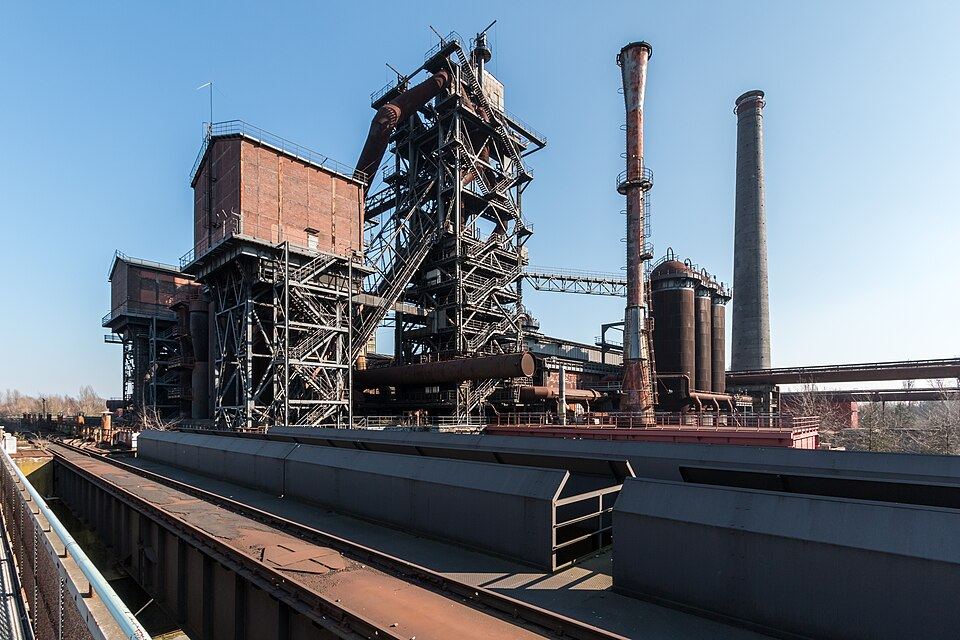
\includegraphics[width=0.6\linewidth]{images/book3/blast-furnace.jpg}

{\small A blast furnace preserved as a monument (Duisburg-Nord, shut down in
1985): the tall shaft with its ring of pipes for the hot air, the gas off-takes
at the top. (Photograph: Dietmar Rabich, CC BY-SA 4.0, Wikimedia Commons.)}
\end{omfigure}

\section{Other routes to a metal}

\begin{definition}[Pyrometallurgy and hydrometallurgy]\label{def:b2:ellingham:metallurgy}
\emph{Pyrometallurgy}\index{pyrometallurgy} extracts a metal at high
temperature, by reduction of its oxide in a furnace. \emph{Hydrometallurgy}\index{hydrometallurgy}
extracts it from an aqueous solution. Their usual steps are
\emph{roasting}\index{roasting} (heating a sulfide ore in air to turn it into
an oxide, \ce{2ZnS + 3O2 -> 2ZnO + 2SO2}), \emph{leaching}\index{leaching}
(dissolving the metal's compound, often in sulfuric acid, \ce{ZnO + 2H+ ->
Zn^2+ + H2O}), purification of the solution, for instance by
\emph{cementation}\index{cementation} (reduction of the ions of a nobler metal
by a powder of a less noble one, \ce{Cu^2+ + Zn -> Cu + Zn^2+}), and the
recovery of the metal, often by electrolysis.
\end{definition}

The diagram explains the division of labour. Iron, zinc, lead, tin are won by
carbon in a furnace. Aluminium, whose line lies far below that of carbon at any
practicable temperature, is made by electrolysis of its molten oxide
(\cref{ch:b2:batteries-electrolysis}); magnesium by electrolysis or by
reduction with silicon under vacuum, which removes the magnesium vapour;
titanium by converting the oxide to the chloride, \ce{TiO2 + 2Cl2 + C -> TiCl4 +
CO2} (\cref{exo:b2:reaction-free-energy:12}), then reducing the chloride with
magnesium (the Kroll process). Most of the world's zinc is made by \omterm{def:b2:ellingham:metallurgy}{roasting},
\omterm{def:b2:ellingham:metallurgy}{leaching} and electrolysis: the hydrometallurgical route gives a purer metal and
avoids handling zinc vapour.

\begin{omfigure}
\begin{tikzpicture}[font=\small, >={Stealth}, box/.style={draw, thick, rounded corners=2pt, align=center, minimum height=0.9cm, fill=white, text width=2.3cm}]
  \node[box] (r) at (0,0) {roasting\\ \ce{ZnS} $\to$ \ce{ZnO}};
  \node[box] (l) at (3.2,0) {leaching\\ in \ce{H2SO4}};
  \node[box] (c) at (6.4,0) {purification\\ (cementation)};
  \node[box] (e) at (9.6,0) {electrolysis\\ \ce{Zn^2+} $\to$ \ce{Zn}};
  \draw[->, thick] (r) -- (l); \draw[->, thick] (l) -- (c); \draw[->, thick] (c) -- (e);
  \draw[->, thick, black!60] (r.north) -- ++(0,0.7) node[above] {\ce{SO2} $\to$ sulfuric acid};
  \draw[->, thick, omThm] (e.south) -- ++(0,-0.6) -| (l.south) node[pos=0.25, below] {acid returned};
  \draw[->, thick] (e.east) -- ++(0.8,0) node[right] {zinc};
\end{tikzpicture}

{\small The hydrometallurgical route to zinc. The sulfur dioxide of the roaster
is made into the sulfuric acid of the leach; the acid regenerated at the
electrolysis anode is returned to it.}
\end{omfigure}

\section{Exercises}

\begin{exercise}[$\star$]\label{exo:b2:ellingham:1}
Write the reactions represented by the lines of copper(I) oxide, alumina, carbon
monoxide and carbon dioxide, each for one mole of \ce{O2}.
\end{exercise}

\begin{exercise}[$\star$]\label{exo:b2:ellingham:2}
From the CODATA key values ($\Delta_f H^\circ(\ce{ZnO}) = \qty{-350.46}{kJ/mol}$,
$S^\circ$: \ce{ZnO} 43.65, \ce{Zn} 41.63, \ce{O2} \qty{205.15}{J/(K.mol)}),
write $\Delta_r G^\circ(T)$ of \ce{2Zn + O2 -> 2ZnO} for solid zinc.
\end{exercise}

\begin{exercise}[$\star$]\label{exo:b2:ellingham:3}
Using the diagram, list the metals that can reduce chromium(III) oxide at
\qty{1500}{K}, and those that cannot.
\end{exercise}

\begin{exercise}[$\star$]\label{exo:b2:ellingham:4}
Explain the sign of the slope of each of the three carbon lines.
\end{exercise}

\begin{exercise}[$\star\star$]\label{exo:b2:ellingham:5}
Compute the \omterm{def:b2:ellingham:oxygen-pressure}{equilibrium oxygen pressure} of mercury(II) oxide at \qty{600}{K}
(mercury liquid, $\Delta_r H^\circ = \qty{-181.6}{kJ}$, $\Delta_r S^\circ =
\qty{-216.5}{J/K}$ per mole of \ce{O2}). Is mercury oxidised in air at that
temperature?
\end{exercise}

\begin{exercise}[$\star\star$]\label{exo:b2:ellingham:6}
Compute $\Delta_r G^\circ$ at \qty{298}{K} of the thermite reaction, \ce{Fe2O3 +
2Al -> Al2O3 + 2Fe}, given $\Delta_f G^\circ = \qty{-743.5}{kJ/mol}$ for
\ce{Fe2O3} and \qty{-1582.3}{kJ/mol} for \ce{Al2O3}, and say why the reaction,
though very \omterm{def:b2:reaction-free-energy:exergonic}{exergonic}, does not start at room temperature.
% ledger: janafG:Fe2O3.298, janafG:Al2O3.298
\end{exercise}

\begin{exercise}[$\star\star$]\label{exo:b2:ellingham:7}
Find on the diagram the temperature above which carbon reduces iron(II) oxide
to iron with formation of carbon monoxide, and write the reaction.
\end{exercise}

\begin{exercise}[$\star\star$]\label{exo:b2:ellingham:8}
At \qty{1100}{K}, $\Delta_f G^\circ(\ce{CO}) = \qty{-209.1}{kJ/mol}$ and
$\Delta_f G^\circ(\ce{CO2}) = \qty{-396.0}{kJ/mol}$. Compute $K^\circ$ of the
\omterm{def:b2:ellingham:boudouard}{Boudouard equilibrium} and the mole fraction of carbon monoxide over carbon at
\qty{1}{bar}. What happens to the gas, in contact with soot or iron, when it is
cooled to \qty{700}{K}?
% ledger: janafG:CO.1100, janafG:CO2.1100
\end{exercise}

\begin{exercise}[$\star\star$]\label{exo:b2:ellingham:9}
Hydrogen is sometimes used to reduce tungsten oxide. Using the line of water,
explain why hydrogen is a better reductant than carbon monoxide at high
temperature but a worse one at low temperature.
\end{exercise}

\begin{exercise}[$\star\star\star$]\label{exo:b2:ellingham:10}
Magnesium oxide can be reduced by silicon, \ce{2MgO + Si -> SiO2 + 2Mg}, though
the line of silica lies above that of magnesia at every temperature of the
diagram. At \qty{1500}{K}, magnesium is a gas and the tables give, per mole of
\ce{O2}, \qty{-845.5}{kJ} for magnesia and \qty{-643.7}{kJ} for silica.
Compute $\Delta_r G^\circ$ of the reduction, then the pressure of magnesium
vapour below which it runs forward. How does a vacuum furnace use this?
% ledger: janafG:MgO.1500, janafG:SiO2.1500
\end{exercise}

\begin{exercise}[$\star\star\star$]\label{exo:b2:ellingham:11}
Compute the \omterm{def:b2:equilibrium-shifts:variance}{variance} of the system \ce{FeO(s)}, \ce{Fe(s)}, \ce{CO(g)},
\ce{CO2(g)} at equilibrium. What does it mean for the gas leaving the upper part
of a blast furnace?
\end{exercise}

\begin{exercise}[$\star\star\star$]\label{exo:b2:ellingham:12}
Copper is purified from its leach solution by \omterm{def:b2:ellingham:metallurgy}{cementation} with iron scrap.
Using the standard potentials of the Year 1 volume ($E^\circ(\ce{Cu^2+}/\ce{Cu})
= \qty{0.34}{V}$, $E^\circ(\ce{Fe^2+}/\ce{Fe}) = \qty{-0.41}{V}$), compute the
equilibrium constant of \ce{Cu^2+ + Fe -> Cu + Fe^2+} and the residual
concentration of copper ions when the solution holds \qty{1.0}{mol/L} of
\ce{Fe^2+}.
\end{exercise}

\section{Problem: Zinc by Fire}

\begin{problem}[{Weekend problem --- the Ellingham lines of zinc oxide and of
carbon monoxide, the temperature at which carbon reduces zinc oxide, the
variance of the furnace, and the condensation of zinc vapour}]
\label{pb:b2:ellingham:1}
Before electrolysis, zinc was made by heating its oxide with carbon in clay
retorts. Data (CODATA, and the JANAF table of zinc): $\Delta_f H^\circ(\ce{ZnO})
= \qty{-350.46}{kJ/mol}$; $S^\circ$ (\unit{J/(K.mol)}): \ce{ZnO} 43.65, \ce{Zn}
41.63, \ce{O2} 205.15; zinc melts at \qty{692.7}{K} ($\Delta_{\text{fus}}H =
\qty{7.32}{kJ/mol}$) and boils at \qty{1180.2}{K} under \qty{1}{bar}
($\Delta_{\text{vap}}H = \qty{115.3}{kJ/mol}$). For \ce{2C + O2 -> 2CO}, the
tables give $\Delta_r G^\circ = \qty{-418.2}{kJ}$ at \qty{1100}{K} and
\qty{-453.0}{kJ} at \qty{1300}{K}.
% ledger: dfh:ZnO_cr, s0:ZnO_cr, s0:Zn_cr, s0:O2_g, hT:Zn_cr.692, hT:Zn_l.692, hT:Zn_l.1180, hT:Zn_g.1180, dfh:Zn_g, janafG:CO.1100, janafG:CO.1300

\medskip
\noindent\textbf{Part I --- The line of zinc oxide.}
\begin{enumerate}
  \item Compute $\Delta_r H^\circ$ and $\Delta_r S^\circ$ of \ce{2Zn(s) + O2 ->
        2ZnO} at \qty{298}{K}.
  \item Write $\Delta_r G^\circ(T)$ below the melting point.
  \item Compute the entropies of fusion and of vaporisation of zinc.
  \item Write $\Delta_r G^\circ(T)$ between the melting and the boiling points.
  \item Write it above the boiling point.
  \item Compute the three slopes and explain why the last is much steeper.
  \item Check that the three expressions agree at the transition temperatures.
\end{enumerate}

\medskip
\noindent\textbf{Part II --- The carbon line.}
\begin{enumerate}[resume]
  \item From the two tabulated values, write the line of \ce{2C + O2 -> 2CO} in
        the form $a + bT$ between \qty{1100}{K} and \qty{1300}{K}.
  \item Deduce its $\Delta_r S^\circ$ and explain its sign.
  \item Write the reduction \ce{ZnO + C -> Zn(g) + CO} and its $\Delta_r
        G^\circ(T)$ as a difference of the two lines (per mole of \ce{O2}).
  \item Find the temperature where the two lines cross.
  \item Why is it important that this temperature is above the boiling point
        of zinc?
\end{enumerate}

\medskip
\noindent\textbf{Part III --- The retort.}
\begin{enumerate}[resume]
  \item Compute the \omterm{def:b2:equilibrium-shifts:variance}{variance} of the system \ce{ZnO(s)}, \ce{C(s)}, \ce{Zn(g)},
        \ce{CO(g)}, with zinc and carbon monoxide formed only by the reduction.
  \item In a retort at \qty{1300}{K} under \qty{1}{bar}, what are the partial
        pressures of zinc and carbon monoxide if the reaction is complete?
  \item Compute $\Delta_r G^\circ$ of the reduction at \qty{1300}{K} and the
        corresponding $K^\circ$.
  \item Explain why the retort is operated slightly above the crossing
        temperature and not far above it.
\end{enumerate}

\medskip
\noindent\textbf{Part IV --- The condenser.}
\begin{enumerate}[resume]
  \item The vapour is led into a cooler condenser. Write the reaction by which
        zinc vapour can be reoxidised by carbon dioxide.
  \item Using the diagram, explain why the gas must be kept free of carbon
        dioxide.
  \item Why must the zinc be condensed quickly rather than slowly?
  \item Compute the mass of carbon needed per tonne of zinc, taking the
        reduction as written.
  \item Compute the heat absorbed per tonne of zinc by the reduction at about
        \qty{1300}{K} (take $\Delta_r H^\circ$ from the expressions of Parts I
        and II).
  \item State the temperature above which carbon reduces zinc oxide under
        standard conditions.
\end{enumerate}
\end{problem}
